%%%%%%%%%%%%%%%%%%%%%%%%%%%%%%%%%%%%%%%%%
% Beamer Presentation
% LaTeX Template
% Version 1.0 (10/11/12)
%
% This template has been downloaded from:
% http://www.LaTeXTemplates.com
%
% License:
% CC BY-NC-SA 3.0 (http://creativecommons.org/licenses/by-nc-sa/3.0/)
%
%%%%%%%%%%%%%%%%%%%%%%%%%%%%%%%%%%%%%%%%%

%----------------------------------------------------------------------------------------
%	PACKAGES AND THEMES
%----------------------------------------------------------------------------------------

\documentclass{beamer}

\mode<presentation> {

% The Beamer class comes with a number of default slide themes
% which change the colors and layouts of slides. Below this is a list
% of all the themes, uncomment each in turn to see what they look like.

%\usetheme{default}
%\usetheme{AnnArbor}
%\usetheme{Antibes}
%\usetheme{Bergen}
%\usetheme{Berkeley}
%\usetheme{Berlin}
%\usetheme{Boadilla}
%\usetheme{CambridgeUS}
%\usetheme{Copenhagen}
%\usetheme{Darmstadt}
%\usetheme{Dresden}
%\usetheme{Frankfurt}
%\usetheme{Goettingen}
%\usetheme{Hannover}
%\usetheme{Ilmenau}
%\usetheme{JuanLesPins}
%\usetheme{Luebeck}
\usetheme{Madrid}
%\usetheme{Malmoe}
%\usetheme{Marburg}
%\usetheme{Montpellier}
%\usetheme{PaloAlto}
%\usetheme{Pittsburgh}
%\usetheme{Rochester}
%\usetheme{Singapore}
%\usetheme{Szeged}
%\usetheme{Warsaw}

% As well as themes, the Beamer class has a number of color themes
% for any slide theme. Uncomment each of these in turn to see how it
% changes the colors of your current slide theme.

%\usecolortheme{albatross}
%\usecolortheme{beaver}
%\usecolortheme{beetle}
%\usecolortheme{crane}
%\usecolortheme{dolphin}
%\usecolortheme{dove}
%\usecolortheme{fly}
%\usecolortheme{lily}
%\usecolortheme{orchid}
%\usecolortheme{rose}
%\usecolortheme{seagull}
%\usecolortheme{seahorse}
%\usecolortheme{whale}
%\usecolortheme{wolverine}

%\setbeamertemplate{footline} % To remove the footer line in all slides uncomment this line
%\setbeamertemplate{footline}[page number] % To replace the footer line in all slides with a simple slide count uncomment this line

%\setbeamertemplate{navigation symbols}{} % To remove the navigation symbols from the bottom of all slides uncomment this line
}

\usepackage{graphicx} % Allows including images
\usepackage{booktabs} % Allows the use of \toprule, \midrule and \bottomrule in tables
\usepackage{multirow}
\usepackage{adjustbox}
\usepackage{array}
\usepackage{tikz}
\usepackage{soul}
\usetikzlibrary{shapes.geometric, arrows, positioning, fit}
\usepackage[latin1]{inputenc}
\newcommand{\xmark}{\textcolor{red}{\text{\sffamily X}}}
\newcommand{\cmark}{\textcolor{green}{\checkmark}}
\newcommand{\tr}{\text{tr}}
\newcommand{\E}{\textbf{E}}
\newcommand{\diag}{\text{diag}}
\newcommand{\argmax}{\text{argmax}}
\newcommand{\argmin}{\text{argmin}}
\newcommand{\Cov}{\text{Cov}}
\newcommand{\Var}{\text{Var}}
\newcommand{\Vol}{\text{Vol}}
\newcommand{\bx}{\boldsymbol{x}}
\newcommand{\by}{\boldsymbol{y}}
\newcommand{\bX}{\boldsymbol{X}}
\newcommand{\bY}{\boldsymbol{Y}}
\sethlcolor{gray}
\makeatletter
\newcommand\SoulColor{%
  \let\set@color\beamerorig@set@color
  \let\reset@color\beamerorig@reset@color}
\makeatother
\definecolor{color1}{RGB}{128,13,13}
\definecolor{color2}{RGB}{70,128,13}
\definecolor{color3}{RGB}{13,128,128}
\definecolor{color4}{RGB}{70,13,128}

%tikz stufff


%----------------------------------------------------------------------------------------
%	TITLE PAGE
%----------------------------------------------------------------------------------------


\title[Mutual information]{Estimating mutual information using sparse regression}

\author{Charles Zheng} % Your name
\institute[Stanford] % Your institution as it will appear on the bottom of every slide, may be shorthand to save space
{Stanford University}
\date{\today} % Date, can be changed to a custom date

\begin{document}

\begin{frame}
\titlepage % Print the title page as the first slide
(Joint work with Yuval Benjamini.)
\end{frame}


\section{Introduction}

\begin{frame}
\frametitle{Mutual information (Shannon 1948)}
\begin{center}
\includegraphics[scale = 0.2]{kinney.png}
\end{center}
\begin{itemize}
\item $I(X;Y) \in [0,\infty]$.  (0 if $X \perp Y$, $\infty$ if $X=Y$ and $X$ continuous.)
\item Symmetry: $I(X;Y) = I(Y; X)$.
\item Data-processing inequality
\[I(X; Y) \geq I(\phi(X); \psi(Y))\]
equality for $\phi$, $\psi$ bijections
%\item Additivity.  If $(X_1,Y_1) \perp (X_2, Y_2)$, then
%\[
%I((X_1, X_2); (Y_1, Y2)) = I(X_1; Y_1) + I(X_2; Y_2).
%\]
%\item Relation to KL divergence
%\[\mathbb{D}(p(x, y)||p(x)p(y)) = I(X; Y).\]
\end{itemize}
\tiny{Image credit Kinney et al. 2014.}
\end{frame}

\begin{frame}
\frametitle{Applications of $I(X; Y)$} 
\begin{itemize}
\item Feature selection (Peng et al. 2005, Fleuret 2004, Bennesar et al. 2015)
\item Structure learning for graphical models using conditional mutual information $I(X; Y|Z)$
(Vastano and Swinney 1988, Cheng et al. 1997, Bach and Jordan 2002)
\item Quantifying information capacity of neurons
\begin{center}
\includegraphics[scale = 0.2]{quiroga.png}
\end{center}
\tiny{Image credits: Quiroga et al. (2009).}
\end{itemize}
\end{frame}

\begin{frame}
\frametitle{How to estimate $I(X; Y)$}
Suppose we observe pairs $(X_i,Y_i)_{i=1}^n$ iid from density $p(x, y)$
\begin{itemize}
\item Definition of mutual information:
\[
I(X; Y) = \int \log \left(\frac{p(x, y)}{p(x)p(y)}\right) p(x, y) dx dy
\]
\item Simply using plugging in kernel density estimate $\hat{p}(x, y)$ leads to large bias (Beirlant et al. 2001)
\item Jackknifed estimate gives better result (Ivanov and Rozhkova 1981)
\[
\hat{I}(X; Y) = \frac{1}{n} \sum_{i=1}^n \log \left(\frac{\hat{p}_{-i}(x_i, y_i)}{\hat{p}_{-i}(x_i)\hat{p}_{-i}(y_i)}\right)
\]
\end{itemize}
\end{frame}

\begin{frame}
\frametitle{Problems in high dimensions}
\begin{itemize}
\item Density estimation is known to have exponential complexity with respect to dimensionality.
\item Many applications with high-dimensional $X$, $Y$.
\begin{itemize}
\item Gene expression time series
\item Functional magnetic resonance imaging
\end{itemize}
\item One approach is to assume joint multivariate normality of $X$, $Y$, but this reduces mutual information to a linear statistic.
\item Other approaches: binning (Bialek et al. 1991, Paninski 2003), confusion matrix of a classifier (Treves 1997, Quiroga et al. 2009).
\end{itemize}
\end{frame}


\begin{frame}
\frametitle{Idea: Use sparsity!}
\begin{center}
\includegraphics[scale = 0.05]{sls.jpg}
\end{center}
\begin{itemize}
\item Suppose that $Y \approx f(X) + \epsilon$, where $f$ depends \emph{sparsely} on $X$.
\item Can we exploit the sparsity to obtain an estimate of $I(X; Y)$?
\end{itemize}
\end{frame}


\begin{frame}
\frametitle{Our proposal}
Suppose we observe pairs $(X_i,Y_i)_{i=1}^n$ iid from density $p(x, y)$.
\begin{enumerate}
\item Estimate a (sparse) regression model for $\E[y|x]$.
\item Estimate the noise model for $Y$.
\item Estimate the \emph{identification risk} $p$ using cross-validation.
\item Use the identification risk to obtain a lower bound for the mutual information $I(X; Y)$:
\[
I(X; Y) \geq f(p)
\]
where $f$ is a function that we derive theoretically. 
\end{enumerate}
\end{frame}

\begin{frame}
\frametitle{Multiple-response regression}
\begin{itemize}
\item Pairs $(x_i,y_i)_{i=1}^n$, where $X$ is $p$-dimensional and $Y$ is $q$-dimensional.
\item Data matrices $\bX_{n \times p}$, $\bY_{n \times q}$.
\item For each column of $Y$, fit sparse model $Y^{(i)} \approx X^T \beta^{(i)}  + \epsilon$, e.g. by using elastic net (Zou 1998), 
\[
\hat{\beta}^{(i)} = \text{argmin}_\beta ||\bX^T \beta^{(i)} - Y^{(i)}||^2 + \lambda_2 ||\beta^{(i)}||_2^2 + \lambda_1 ||\beta^{(i)}||_1
\]
\item Or, fit a \emph{random forest} model for each column of $Y$ (Breiman 2001)
\end{itemize}
\end{frame}


\begin{frame}
\frametitle{Regression vs Identification loss}
\begin{itemize}
\item Independent \emph{test set} $(x_i^*, y_i^*)_{i=1}^k$. 
\item Use model to predict $\hat{y}_i^* = (x_i^*)^T \hat{B}$ for $i = 1,\hdots, k$.
\end{itemize}
Two ways to evaluate the predictive accuracy of the regression model:
\begin{itemize}
\item Regression (mean squared-error) loss:
\[
\text{MSE} = \frac{1}{k} \sum_{i=1}^k ||y_i^* - \hat{y}_i^*||^2.
\]
\item Identification loss:
\[
\text{IdLoss}_k = \frac{1}{k} \sum_{i=1}^k (1 - I\{\hat{y}_i^* \text{ is nearest neighbor of }y_i^*\}).
\]
\end{itemize}
\end{frame}

\begin{frame}
\frametitle{Cross-validated loss}
Leave-$k$-out cross-validation (L$k$oCV) can be used for both squared-error loss and identification loss.
\begin{itemize}
\item Start with a dataset $(x_i,y_i)_{i=1}^N$.
\item Let $n = N-k$.  Consider all ${N}\choose{k}$ partitions of the dataset into a test set $(\bX, \bY)$ and training set $(\bX^*, \bY^*)$.
\item For each partition, compute the loss.
\item Define the L$k$oCV loss as the average loss over ${N}\choose{k}$ partitions.
\end{itemize}
\emph{Computational note}.  One can subsample to avoid computing all
${N}\choose{k}$ partitions.  In particular, if $m = N/k$, then one can
use $m$-fold cross-validation which uses $m$ partitions that have
disjoint test sets.
\end{frame}

\begin{frame}
\frametitle{Identification loss and mutual information}
\begin{itemize}
\item Define the identification risk as the expected identification loss
\[
\text{IdRisk}_k = \E[\text{IdLoss}_k]
\]
\item Define the Bayes risk as the identification risk given the \emph{true} model parameters.
Hence,
\[
\text{BayesRisk}_k \leq \text{IdRisk}_k.
\]
%\item \textbf{High-dimensional result.}  In a certain high-dimensional
%  asymptotic regime, there exists a limiting functional relationship
%\[
%\text{Bayes risk} = \pi_k(\sqrt{2 I(X; Y)})
%\]
\item \textbf{Theorem.} (Z., Benjamini 2016) There exists a function $g_k$ such that
%For every $k \geq 2$, there exists a function $g_k$ such that
\[I(X; Y) \geq g_k(\text{IdRisk}_k).\]
%$\Box$.
\item Resulting estimator:
\[
\hat{I}_{IdLoss}(X; Y) = g_k(\text{IdLoss}_k)).
\]
%\item \emph{Remark.} Although $\text{IdLoss}_k$ is unbiased for $\text{IdRisk}_k$, $g_k$ is nonlinear so $\hat{I}_{IdLoss}$ may be biased.
\end{itemize}
\end{frame}

\begin{frame}
\frametitle{Functions}

Illustration of $C_k = g_k^{-1}$
\begin{center}
\includegraphics[scale = 0.34]{ck_2.pdf}
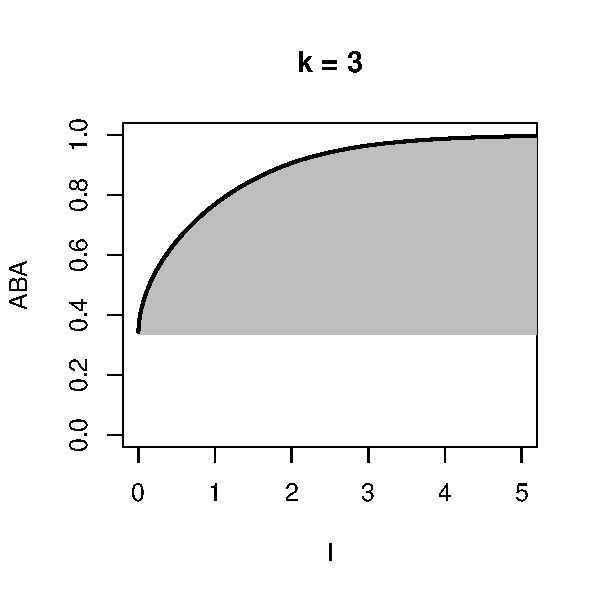
\includegraphics[scale = 0.34]{ck_3.pdf}
\includegraphics[scale = 0.34]{ck_4.pdf}
\end{center}
As information increases, the maximal identification risk goes to 0.
[note: pictures need to be rotated]
%We find these curves using \emph{variational calculus}.

\end{frame}

\section{Applications}

\begin{frame}
\sectionpage
\end{frame}

\begin{frame}
\frametitle{Simulation}


\begin{center}
\includegraphics[scale = 0.34]{../idloss/sim1_pairs.pdf}
\end{center}
\begin{itemize}
\item Generate data: $(Y_1, Y_2) = f(X_1, X_2, \epsilon)$ where $f$ is nonlinear.
\item $n = 1000$.
\item Compare Nearest-Neighbor estimator (Mnatsakov et al, 2008, implemented in {\tt FNN}) with our method using \emph{Random Forest}.
\item Add extra noise dimensions $X_3, X_4, \hdots$.
\end{itemize}

%We find these curves using \emph{variational calculus}.

\end{frame}

\begin{frame}
\frametitle{Simulation Results}

True $I(X; Y) = 4.615$.

\begin{center}
\begin{tabular}{c||c|c|c}
Extra dim & NN & RF $k = 10$ & RF $k=20$\\
0 & \textbf{4.445} & 3.989 & 3.924\\
1 & 3.040 & \textbf{3.645} & 3.610\\
2 & 1.773 & \textbf{3.249} & 3.182
\end{tabular}
\end{center}

%We find these curves using \emph{variational calculus}.

\end{frame}

\begin{frame}
\frametitle{Application to gene expression time series}
to be contd
\end{frame}

\section{Theory}

\begin{frame}
\sectionpage
\end{frame}


\begin{frame}
\frametitle{Functional formulation}
Bayes identification risk $\text{BayesRisk}_k[p(x, y)]$ and mutual information $\text{I}[p(x, y)]$ are both \emph{functionals} of $p(x, y)$.
\[
\text{BayesAcc}_k[p(x, y)] = 1 - \frac{1}{k} \int p_X(x_1)\hdots p_X(x_k) \max_{i=1}^k p(y|x_i)  dx_1\hdots dx_k dy.
\]
\[
\text{I}[p(x, y)] = \int p(x, y) \log \frac{p(x, y)}{p(x)p(y)} dx dy.
\]
where $\text{BayesAcc}_k = 1 - \text{BayesRisk}_k$.
\end{frame}

\begin{frame}
\frametitle{Problem formulation} Take $\iota > 0$, and fix $k \in
\{2,3,...\}$.  Let $p(x, y)$ be a joint density (where $(X, Y)$
could be random vectors of any dimensionality.)  Supposing
\[
\text{I}[p(x, y)] \leq \iota,
\]
then can we find an upper bound on $\text{BayesAcc}_k[p(x, y)]$?

\end{frame}

\begin{frame}
\frametitle{Proof outline}
\begin{enumerate}
\item Reduce problem to optimization over univariate densities.
\item Define the Lagrangian functional
\[
\mathcal{L}[q(x)] = -\text{BayesAcc}_k[q(x)] + \lambda \int_0^1 q(x) dx + \nu \text{I}[q(x)]
\]
which maps the univariate density $q(x)$ to a real number.
\item Compute the functional derivative of the Lagrangian
\[
\nabla \mathcal{L}[q](x) = -t^{k-1} + \lambda + \nu (1 + \log q(x))
\]
\item Set $\nabla \mathcal{L}[q](x) = 0$, yielding
\[
q^*(t) = \alpha e^{\beta t^{k-1}}.
\]
\item Check that local minimizer is global minimizer.
\end{enumerate}
\end{frame}

\begin{frame}
\frametitle{Result}
\textbf{Theorem}.
For any $\iota > 0$, there exists $\beta_\iota \geq 0$ such that defining
\[
q_\beta(t) = \frac{\exp[\beta t^{k-1}]}{\int_0^1 \exp[\beta t^{k-1}]},
\]
we have
\[
\int_0^1 q_{\beta_\iota}(t) \log q_{\beta_\iota}(t) dt = \iota.
\]
Then,
\[
\sup_{I(X; Y) = \iota} \text{BayesAcc}_k = \int_0^1 q_{\beta_\iota}(t) t^{k-1} dt.
\]
\end{frame}

\section{The End}

\begin{frame}
\sectionpage
\end{frame}


\begin{frame}
\frametitle{Reduced Problem}
Rather than show the whole proof, we consider a simplified problem to illustrate the methods.
\begin{center}
\includegraphics[scale = 0.5]{../diagram/qxplot.png}
\end{center}

Actually, the simplified problem is equivalent to the full problem and we get the same answer (but this is non-trivial).
\end{frame}

\begin{frame}
\frametitle{Reduced Problem}

\begin{center}
\includegraphics[scale = 0.4]{../diagram/qxplot.png}
\end{center}

\begin{itemize}
\item $p(x, y)$ on unit square with uniform marginals.
\item The conditional distributions $p(x|y)$ are just ``shifted'' copies of a common density, $q(x)$, on $[0,1]$
\[
p(x|y) = q(x - y + I\{x < y\})
\]
\item Furthermore, $q(x)$ is increasing in $x$.
\end{itemize}

\end{frame}

\begin{frame}
\frametitle{Simplified formulae}

The information and average Bayes error can be written in terms of $q(x)$.

\[
\text{I}[p(x, y)] = \int_0^1 q(x) \log q(x) dx
\]
\[
\text{BayesAcc}_k[p(x, y)] = \int_{[0, 1]^k} \max_{i=1}^k q(x_i) dx_1 \cdots dx_k
\]



\end{frame}

\begin{frame}
\frametitle{Simplified formulae}

Overload the notation and ``redefine'' information and average Bayes error as functionals of $q(x)$.

\[
\text{I}[q(x)] \stackrel{def}{=} \int_0^1 q(x) \log q(x) dx
\]
\[
\text{BayesAcc}_k[q(x)] \stackrel{def}{=} \frac{1}{k}\int_{[0, 1]^k} \max_{i=1}^k q(x_i) dx_1 \cdots dx_k
\]

\end{frame}

\begin{frame}
\frametitle{Optimization problem}
We now pose the question: how do we find $q(x)$ which maximizes $\text{BayesAcc}_k[q(x)]$ subject to $\text{I}[q(x)] \leq \iota$?

\begin{itemize}
\item \emph{Domain of the optimization}: Recall that $q(x)$ satisfies $q(x) \geq 0$, $\int_0^1 q(x) dx = 1$, and is increasing in $x$.
Let $\mathcal{Q}$ denote the space of functions on $[0,1] \to [0,\infty)$ which are increasing in $x$.
\item \emph{Constraints}: We have two remaining constraints, $\text{I}[q(x)] \leq \iota$ and $\int_0^1 q(x) dx = 1$.
\end{itemize}

Hence the problem is
\[
\text{maximize}_{q(x) \in \mathcal{Q}}\text{ BayesAcc}_k[q(x)]\text{ subject to }\int_0^1 q(x) dx = 1\text{ and }\text{I}[q(x)] \leq \iota.
\]
\end{frame}


\begin{frame}
\frametitle{Optimization problem}
\[
\text{maximize}_{q(x) \in \mathcal{Q}}\text{ BayesAcc}_k[q(x)]\text{ subject to }\int_0^1 q(x) dx = 1\text{ and }\text{I}[q(x)] \leq \iota.
\]
\begin{itemize}
\item Does a solution exist? \emph{Yes}, because the space of measures
  with density $q(x)$ satisfying $\text{I}[q(x)] \leq \iota$ is tight,
  and both the constraints and objective are continuous wrt to the
  topology of weak convergence.
\item Given a solution $q^*(x)$ exists, there exist Lagrange multipliers $\lambda \in \mathbb{R}$ and $\nu > 0$ such that $q^*$ minimizes
\begin{align*}
\mathcal{L}[q(x)] &= -\text{BayesAcc}_k[q(x)] + \lambda \int_0^1 q(x) dx + \nu \text{I}[q(x)]
\\&= \int_0^1 (-t^{k-1} + \lambda + \nu \log q(x)) q(x) dx.
\end{align*}
\end{itemize}

\end{frame}

\begin{frame}
\frametitle{Functional derivatives}
\begin{itemize}
\item Taylor explansions are a useful trick for computing functional derivatives
\item We can compute the functional derivative of $\mathcal{L}[q(x)]$ by writing
\begin{align*}
\mathcal{L}[q(x) + \epsilon \xi(x)] &
\\= \int_0^1 (-t^{k-1} &+ \lambda + \nu \log (q(x) + \epsilon \xi(x))) (q(x) + \epsilon \xi(x)) dx.
\\\approx  \int (q(x) + &\epsilon \xi(x)) (-t^{k-1} + \lambda + \nu \{\log q(x) + \frac{\epsilon \xi(x)}{q(x)}\}) dx
\\\approx  \mathcal{L}[q(x)] +& \int_0^1 (-t^{k-1} + \lambda + \nu (1 + \log q(x)) \epsilon\xi(x) dx.
\end{align*}
\item Hence
\[
\nabla \mathcal{L}[q](x) = -t^{k-1} + \lambda + \nu (1 + \log q(x))
\]
\end{itemize}
\end{frame}

\begin{frame}
\frametitle{Variational magic!}
Suppose we set the functional derivative to 0,
\[
0 = \nabla \mathcal{L}[q](t) = -t^{k-1} + \lambda + \nu + \nu \log q(t).
\]
Then we conclude that the optimal $q^*(t)$ takes the form
\[
q^*(t) = \alpha e^{\beta t^{k-1}}
\]
for some $\alpha > 0$, $\beta > 0$.

From the constraint $\int q(t)dt = 1$, we get
\[
q_\beta(t) = \frac{e^{\beta t^{k-1}}}{\int e^{\beta t^{k-1}} dt}.
\]
\end{frame}

\begin{frame}
\frametitle{Result}
\textbf{Theorem}.
For any $\iota > 0$, there exists $\beta_\iota \geq 0$ such that defining
\[
q_\beta(t) = \frac{\exp[\beta t^{k-1}]}{\int_0^1 \exp[\beta t^{k-1}]},
\]
we have
\[
\int_0^1 q_{\beta_\iota}(t) \log q_{\beta_\iota}(t) dt = \iota.
\]
Then,
\[
\sup_{I(X; Y) = \iota} \text{BayesAcc}_k = \int_0^1 q_{\beta_\iota}(t) t^{k-1} dt.
\]
\end{frame}

\end{document}
